% Created by tikzDevice version 0.12.3.1 on 2022-09-04 15:30:55
% !TEX encoding = UTF-8 Unicode
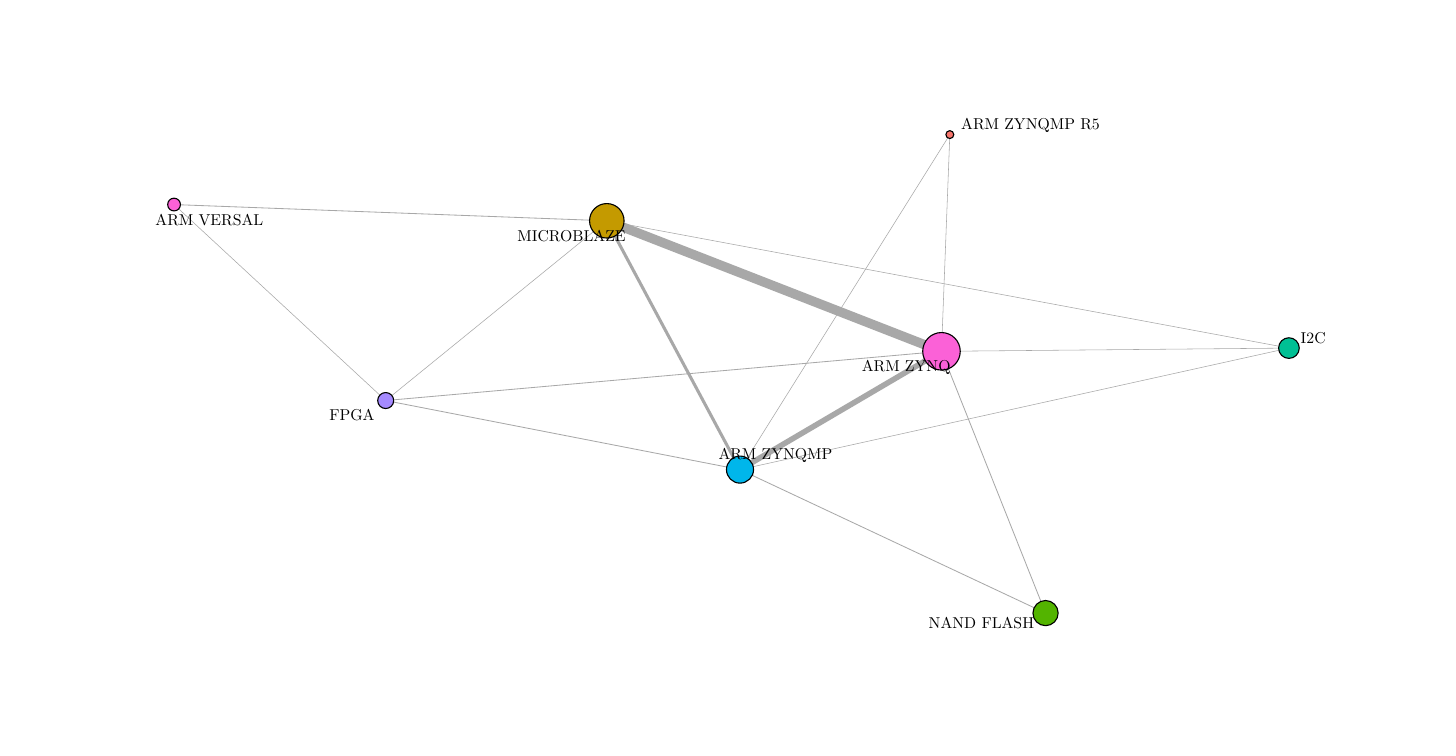
\begin{tikzpicture}[x=1pt,y=1pt]
\definecolor{fillColor}{RGB}{255,255,255}
\path[use as bounding box,fill=fillColor,fill opacity=0.00] (0,0) rectangle (505.89,252.94);
\begin{scope}
\path[clip] (  0.00,  0.00) rectangle (505.89,252.94);
\definecolor{fillColor}{RGB}{255,255,255}

\path[fill=fillColor] (  0.00,  0.00) rectangle (505.89,252.94);
\end{scope}
\begin{scope}
\path[clip] ( 32.75, 32.75) rectangle (475.89,222.94);
\definecolor{drawColor}{gray}{0.66}

\path[draw=drawColor,line width= 0.2pt,line join=round] ( 52.89,189.02) -- (129.37,118.20);

\path[draw=drawColor,line width= 0.3pt,line join=round] ( 52.89,189.02) -- (209.27,183.15);

\path[draw=drawColor,line width= 2.0pt,line join=round] (330.20,135.99) -- (257.40, 93.25);

\path[draw=drawColor,line width= 0.2pt,line join=round] (330.20,135.99) -- (333.22,214.30);

\path[draw=drawColor,line width= 0.3pt,line join=round] (330.20,135.99) -- (129.37,118.20);

\path[draw=drawColor,line width= 0.2pt,line join=round] (330.20,135.99) -- (455.75,137.16);

\path[draw=drawColor,line width= 3.4pt,line join=round] (330.20,135.99) -- (209.27,183.15);

\path[draw=drawColor,line width= 0.3pt,line join=round] (330.20,135.99) -- (367.81, 41.40);

\path[draw=drawColor,line width= 0.2pt,line join=round] (257.40, 93.25) -- (333.22,214.30);

\path[draw=drawColor,line width= 0.3pt,line join=round] (257.40, 93.25) -- (129.37,118.20);

\path[draw=drawColor,line width= 0.2pt,line join=round] (257.40, 93.25) -- (455.75,137.16);

\path[draw=drawColor,line width= 1.1pt,line join=round] (257.40, 93.25) -- (209.27,183.15);

\path[draw=drawColor,line width= 0.3pt,line join=round] (257.40, 93.25) -- (367.81, 41.40);

\path[draw=drawColor,line width= 0.2pt,line join=round] (129.37,118.20) -- (209.27,183.15);

\path[draw=drawColor,line width= 0.2pt,line join=round] (455.75,137.16) -- (209.27,183.15);
\definecolor{drawColor}{RGB}{0,0,0}
\definecolor{fillColor}{RGB}{251,97,215}

\path[draw=drawColor,line width= 0.4pt,line join=round,line cap=round,fill=fillColor] ( 52.89,189.02) circle (  2.30);

\path[draw=drawColor,line width= 0.4pt,line join=round,line cap=round,fill=fillColor] (330.20,135.99) circle (  6.78);
\definecolor{fillColor}{RGB}{0,182,235}

\path[draw=drawColor,line width= 0.4pt,line join=round,line cap=round,fill=fillColor] (257.40, 93.25) circle (  4.89);
\definecolor{fillColor}{RGB}{248,118,109}

\path[draw=drawColor,line width= 0.4pt,line join=round,line cap=round,fill=fillColor] (333.22,214.30) circle (  1.43);
\definecolor{fillColor}{RGB}{165,138,255}

\path[draw=drawColor,line width= 0.4pt,line join=round,line cap=round,fill=fillColor] (129.37,118.20) circle (  2.89);
\definecolor{fillColor}{RGB}{0,192,148}

\path[draw=drawColor,line width= 0.4pt,line join=round,line cap=round,fill=fillColor] (455.75,137.16) circle (  3.73);
\definecolor{fillColor}{RGB}{196,154,0}

\path[draw=drawColor,line width= 0.4pt,line join=round,line cap=round,fill=fillColor] (209.27,183.15) circle (  6.23);
\definecolor{fillColor}{RGB}{83,180,0}

\path[draw=drawColor,line width= 0.4pt,line join=round,line cap=round,fill=fillColor] (367.81, 41.40) circle (  4.55);

\node[text=drawColor,anchor=base,inner sep=0pt, outer sep=0pt, scale=  0.57] at ( 65.66,181.58) {ARM VERSAL};

\node[text=drawColor,anchor=base,inner sep=0pt, outer sep=0pt, scale=  0.57] at (317.45,128.56) {ARM ZYNQ};

\node[text=drawColor,anchor=base,inner sep=0pt, outer sep=0pt, scale=  0.57] at (270.22, 96.79) {ARM ZYNQMP};

\node[text=drawColor,anchor=base,inner sep=0pt, outer sep=0pt, scale=  0.57] at (362.38,216.00) {ARM ZYNQMP R5};

\node[text=drawColor,anchor=base,inner sep=0pt, outer sep=0pt, scale=  0.57] at (117.16,111.03) {FPGA};

\node[text=drawColor,anchor=base,inner sep=0pt, outer sep=0pt, scale=  0.57] at (464.53,138.96) {I2C};

\node[text=drawColor,anchor=base,inner sep=0pt, outer sep=0pt, scale=  0.57] at (196.52,175.72) {MICROBLAZE};

\node[text=drawColor,anchor=base,inner sep=0pt, outer sep=0pt, scale=  0.57] at (344.63, 35.78) {NAND FLASH};
\end{scope}
\end{tikzpicture}
